\documentclass[../main.tex]{subfiles}

\begin{document}


\begin{figure}
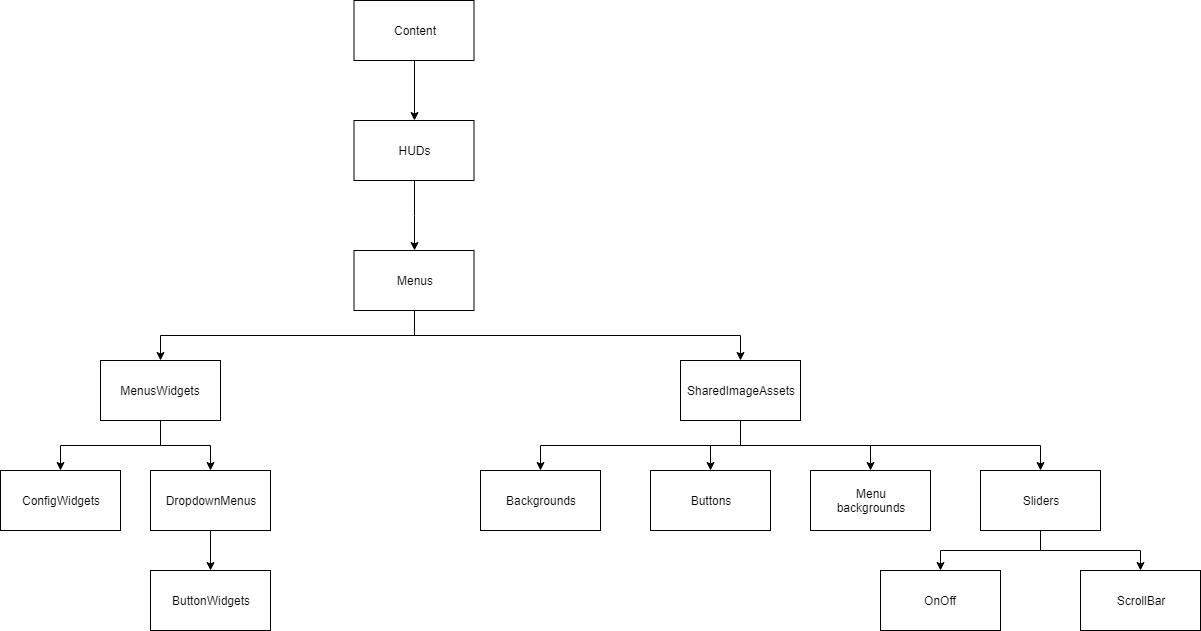
\includegraphics[width=\textwidth,height=\textheight,keepaspectratio]{ContentStructureForMenus.jpg}
\caption{Content Structure}
\end{figure}

\break
\textbf{Assets}
\break
The menus use common assets to allow easier updatability, this is best exemplified by the button background assets. These assets are used by all buttons and allow them to display when a button is either hovered over or not, these assets are located in SharedImageAssets/Buttons.

To add any assets to the project they should be added to the corresponding directory in SharedImageAssets, if necessary a new sub directory should be created. To include a new asset the developer should go to the correct directory and then use the import tool to import the asset.

\begin{figure}
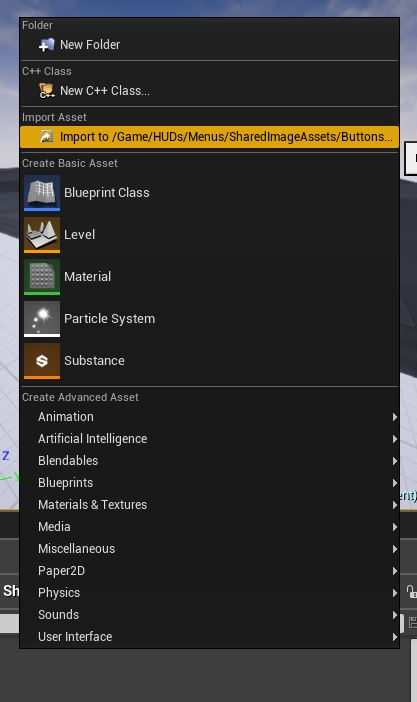
\includegraphics[width=\textwidth,height=\textheight,keepaspectratio]{Importing.jpg}
\caption{Import tool}
\end{figure}

\break
\textbf{Dropdown Menus}
Unreal doesn't have native dropdown menus and so to create a dropdown menu in this project is a bit of a work around. Firstly you have to make a button widget, located in the MenuWidgets/DropdownMenus/ButtonWidgets. You then have to make a new dropdown menu widget, this widget should generate button widgets and have a function on it for the button to reference when the button is clicked. The button widget should then be updated to have a reference to the dropdown widget, calling the dropdown widgets on click function when the button is clicked. By doing this the dropdown menu can react to button clicks of dynamically created buttons.





\end{document}